\documentclass[twocolumn]{ltjarticle}
\usepackage[bibstyle=ieee,citestyle=numeric,maxnames=99,maxnames=2,url=true,doi=true,hyperref=true]{biblatex}
\usepackage[dvipdfmx]{graphicx}
\usepackage{amssymb}
\usepackage{eshouroku}
\usepackage{color}
\usepackage{graphics}
\usepackage{amsmath}
\usepackage{subfigure}
\usepackage{url}
\usepackage{upgreek}
\usepackage{bm}
\usepackage{nicematrix}
\usepackage{enumitem}

\boldmaintrue% 主文を太字にするモード(指導教員添削時はこちら)
% \boldmainfalse% 主文を普通文字にするモード(抄録印刷時はこちら)

\addbibresource{ref.bib}

\begin{document}
\twocolumn[
\講演番号{B-13}% 必要ない場合には書かない
\日本語タイトル{\fontsize{16.1pt}{16.1pt}\selectfont}{通信速度改善のためのベイズ最適化を用いた送信機位置の決定}
\英語タイトル{\large}{Determination of transmitter location using Bayesian optimization for transmission speed improvement}
\筆者一名{5322}{竹中公材}
%\筆者二名{53XX}{産技太郎}{53YY}{品川次郎}
%\筆者三名{53XX}{産技太郎}{53YY}{品川次郎}{53ZZ}{東大井三郎}
%\筆者四名{53XX}{産技太郎}{53YY}{品川次郎}{53ZZ}{東大井三郎}{53WW}{荒川四郎}
\指導教員一名{稲毛契}
%\指導教員二名{東京花子}{京都紀夫}
%\指導教員なし
]

% \addcontentsline{toc}{section}{\refname}% 追加

%\graphicspath{{./figures/}} % 図が特定のフォルダにある場合には設定

\section{はじめに}
私たちが日常的に使用しているスマートフォンやノートパソコンなどの通信機器は持ち運ぶことができ,位置の調整が容易である.
そのため,通信速度が低い場合はその位置を調整することで,通信速度を改善することができる.
しかし,IoT(Internet of Things)の普及に伴い,産業機器や家電製品などに無線通信機能が搭載されることが増えている\cite{soumu}.
これらは複数箇所に固定設置されていることが多く,位置の調整が困難であるため位置変更により通信速度を向上させるのは容易ではない.
このような固定設置された受信機の通信速度を向上させるには,送信機の数を増やす,あるいは高出力の送信機に替えるといった方法が考えられるが,いずれもコスト(送信機の費用)がかかる.

そこで,送信機の位置を調整して受信機の通信速度を向上させる方法が挙げられる.
電波は距離の累乗に比例して減衰するため,送信機と各受信機間の距離から送信機の最適な位置を求める方法が考えられる.
しかし,周囲の構造物による反射や回折により変動が生じ,電波の減衰が複雑になるため通信速度が距離で表せる関数にならず,通信速度の予測が困難になる.
この変動をシャドウイング(短区間変動)と呼ぶ.
そのため,実際に各受信機の通信速度を測定することで最適な位置を決定するのが望ましい.

各受信機の通信速度を測定して送信機の最適な位置を求める方法として,すべての位置のパターンを試す全探査と呼ばれる手法がある.
この手法は,確実に最適な位置を見つけることができるが,多くの試行回数を必要とするため,非常に大きな時間や労力のコストがかかる.

試行回数をできるだけ少なくするためには,送信機の位置を入力,各受信機の中で最も遅い通信速度を出力とする関数と考え,この関数の最大値を求めることが有効である.
しかし,屋内の複雑な電波伝搬特性はブラックボックス関数(具体的な形状が不明な関数)であるため,勾配法やニュートン法などの傾きを用いた最適化を適用することが難しい.

そこで本研究では,ブラックボックス関数でも試行回数を少なくして最適値を求めることができるベイズ最適化と呼ばれる手法を送信機の位置決定に適用し,通信速度を改善することを目的とする.
\section{従来の最適化手法の問題点}

最適化とは,ある関数の最大値や最小値を求めることであり,勾配法やニュートン法などを用いる方法がある.
これらの最適化手法はある関数が\(y=f(x)\)のように数理的な構造が明確であり,傾きを用いるため微分可能であることを前提とする.
しかし,ブラックボックス関数の場合は明確な関数がわからず微分可能か把握できないため,これらの最適化手法を適用できない.
\section{ベイズ最適化}

ブラックボックス関数の最適化には,全探査や粒子群最適化などの方法があるが,これらは試行回数が多くなる.
一方でベイズ最適化は,毎回の測定において適切な入力値を確率的に選択し,少ない試行回数で最適値を効率的に探索する手法であり,
一回あたりの実験コスト(実験費用や時間)が高い場合に有効な手段である.
適切な入力値を確率的に選択するために,ガウス過程回帰を用いる必要がある.
ガウス過程回帰を用いることにより,\wfig{gaussian_process}のように赤点の測定点から関数を正規分布に従う確率分布として推定することができる.
ここで,青線は推定結果(平均\(\mu\)),紫のエリアは68\%の確率で値が存在する区間(標準偏差\(\sigma\))を表す.
ガウス過程回帰では,過去の測定点からカーネル関数を用いて関数の形状を推定する.
そのため,ベイズ最適化ではカーネル関数の選択が重要である.
\setlength\intextsep{3pt}
\setlength\textfloatsep{3pt}
\begin{figure}[htbp]
	\centering
	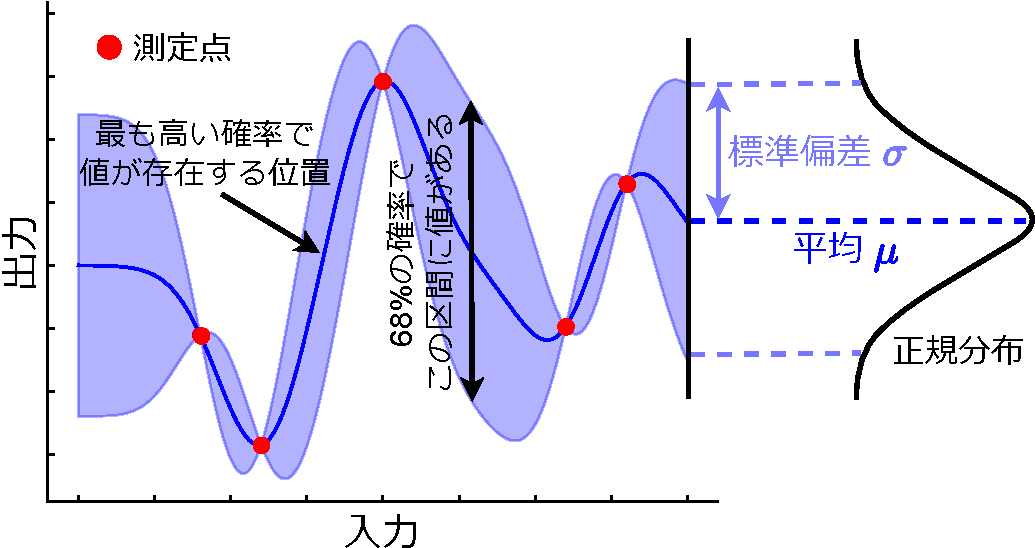
\includegraphics[width=0.83\linewidth]{./figures/material_5_kernel_v2.pdf}
	\vspace*{-0.3cm}
	\caption{ガウスカーネルを用いたガウス過程回帰} \label{fig:gaussian_process}
\end{figure}
\subsection{カーネル関数}

カーネル関数は測定点と測定点がどのような形でつながっているかを示す.
カーネル関数の代表例として,\weq{gaussian_kernel}のようなガウスカーネルがある\cite{gaussian_process}.
\begin{align}
	k(x_a, x_b) = \theta_1 \exp \left( - \frac{\| x_a - x_b \|^2}{\theta_2} \right) \label{eq:gaussian_kernel}
\end{align}
ガウスカーネルにより,\wfig{gaussian_process}のようにガウス関数を用いて測定点と測定点をつなげている.
カーネル関数には,他にも\weq{exp_kernel}や\weq{sin_kernel}のような指数カーネルや周期カーネルがある.
指数カーネルは\wfig{exp_kernel}のように指数関数を用いて測定点と測定点をつなげている.
周期カーネルは\wfig{sin_kernel}のように周期関数を用いて測定点と測定点をつなげている.
\begin{align}
	k(x_a, x_b) & = \theta_1 \exp \left( - \frac{\| x_a - x_b \|}{\theta_2} \right) \label{eq:exp_kernel}                           \\
	k(x_a, x_b) & = \theta_1 \exp \left( \theta_2 \cos \left(\frac{\| x_a - x_b \|}{\theta_3} \right) \right) \label{eq:sin_kernel}
\end{align}
カーネル関数を変更することにより,予測する関数の形状が変化するため,対象とするブラックボックス関数に合わせて適切なカーネル関数を選択する必要がある.
また,カーネル関数は複数のカーネル関数を組み合わせることもでき,指数カーネルと周期カーネルを組み合わせることにより,局所的な特徴をもつ周期関数として回帰することができる.
\setlength\intextsep{6pt}
\setlength\textfloatsep{6pt}
\begin{figure}[htbp]
	\centering
	\begin{minipage}[c]{0.4\columnwidth}
		\centering
		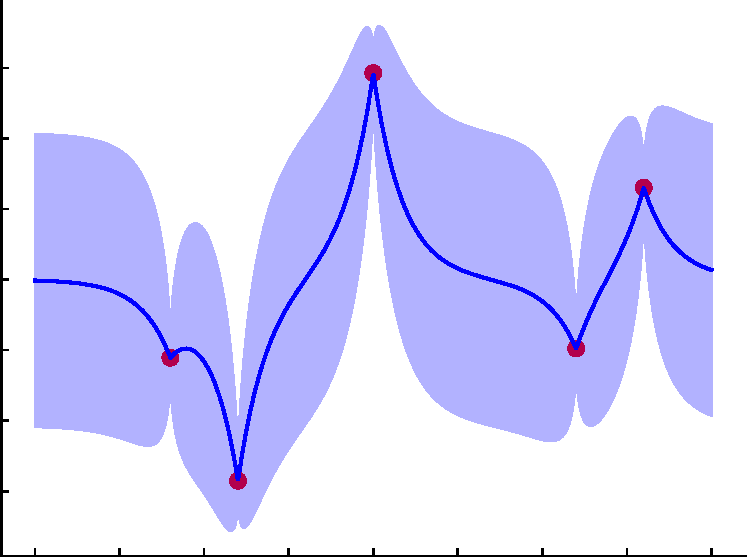
\includegraphics[width=\columnwidth]{figures/gaussian_regression_exp_kernel_crop.pdf}
		\vspace*{-0.6cm}
		\caption{指数カーネル} \label{fig:exp_kernel}
	\end{minipage}
	\hspace{0.05\columnwidth}
	\begin{minipage}[c]{0.4\columnwidth}
		\centering
		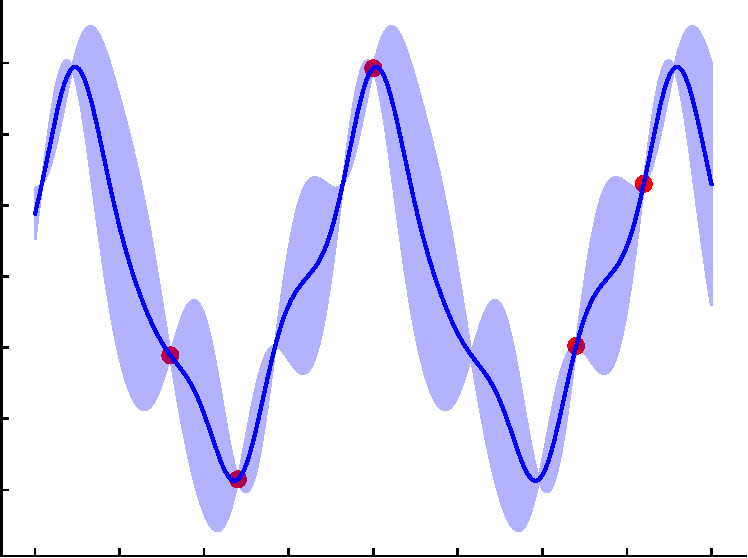
\includegraphics[width=\columnwidth]{figures/gaussian_regression_sin_kernel_crop.pdf}
		\vspace*{-0.6cm}
		\caption{周期カーネル} \label{fig:sin_kernel}
	\end{minipage}
\end{figure}
\subsection{測定手順}

ベイズ最適化では,最初にいくつかの地点を測定する必要がある.
これは,ガウス過程回帰を用いるためにデータが必要であるためである.
次にいくつかの測定データを用いてガウス過程回帰を用い,獲得関数を求める.
獲得関数は,次に測定したら最適値に近づく確率が高い地点を示す関数であり,\weq{acquisition}のように定義される.
ここで,\(\mu\)と\(\sigma\)はそれぞれ平均と標準偏差,\(\beta\)は\(\mu\)と\(\sigma\)を調整するパラメータであり,任意に設定する係数である.
\begin{align}
	a(\mu, \sigma, \beta) = \mu + \beta \sigma \label{eq:acquisition}
\end{align}
\weq{acquisition}で定義した獲得関数の最も高い点を次の測定箇所として選択する.
選択された測定箇所が既に測定されている場合,その地点が最適値となる.
\section{シミュレーション}

ベイズ最適化が送信機の位置決定において有用であるかを確認するために,シミュレーションを行った.
\subsection{関数の作成}

フリスの公式と対数正規シャドウイングを用いて電波伝搬環境を作成し,送信機を動かしながらランダムな場所に配置した複数の受信機の通信速度を計算した.
電波が距離の累乗に比例して減衰する特徴を\weq{friss}のフリスの公式で表現する.
ここで,\(\lambda\,\mathrm{[m]}\)は使用する電波の波長,\(\mathrm{d_0}\,\mathrm{[m]}\)は自由空間距離(遮蔽物に当たらない距離),\(\mathrm{d}\,\mathrm{[m]}\)は送受信機間距離,\(n\)は障害物によりどのぐらい電波が減衰するかを示す伝搬係数である.
\begin{align}
	\scalebox{0.9}{
		\(
		\mathrm{P_{LOSS}} =
		\begin{cases}
			20 \log_{10} \left( \frac{\lambda}{4 \pi \mathrm{d}} \right)                                                         & (\mathrm{d < d_0})     \\
			20 \log_{10} \left( \frac{\lambda}{4 \pi \mathrm{d_0}} \right) - 10n \log_{10} \left( \mathrm{\frac{d}{d_0}} \right) & (\mathrm{d \geqq d_0})
		\end{cases} \label{eq:friss}
		\)
	}
\end{align}

シャドウイングは,空間相関性(距離が近いほど似た値を持つ性質)を表す\weq{shadowing}の相関係数\(\rho\)を用いて相関行列を作成し,
その相関行列をコレスキー分解して得られる下三角行列と正規分布に従う乱数との行列積で表現する\cite{shadowing}.
ここで,\(\mathrm{\Delta d_{TX}}\,\mathrm{[m]}\)は送信機の位置の変化量,\(\mathrm{\Delta d_{RX}}\,\mathrm{[m]}\)は受信機の位置の変化量,\(\mathrm{d_{cor}}\,\mathrm{[m]}\)は位置の変化量によってどのぐらい相関を与えるかを示す相関距離である.
\begin{align}
	\rho \approx \exp \left( - \mathrm{\frac{\Delta d_{TX} + \Delta d_{RX}}{d_{cor}}} \ln 2 \right) \label{eq:shadowing}
\end{align}

\weq{friss}と\weq{shadowing}は受信信号強度(RSSI)を計算する式であるため,\weq{capacity}を用いて受信信号強度から通信速度に変換する必要がある.
ここで,\(\mathrm{RSSI}\,[\mathrm{dBm}]\)は受信信号強度,\(\mathrm{Noise}\,[\mathrm{dBm}]\)はノイズフロア,\(B\,[\mathrm{Hz}]\)は帯域幅,\(C\,[\mathrm{bps}]\)は通信速度である.
\begin{align}
	C = B \log_2 \left( 1 + 10^{\frac{\mathrm{RSSI}}{10}-\frac{\mathrm{Noise}}{10}} \right) \label{eq:capacity}
\end{align}
\subsection{環境}

シミュレーション環境として20\(\,\)m\(\times\)20\(\,\)mの空間を用意し,1台の送信機を作成して1\(\,\)m刻みでグリッド状に設置できるようにした.
また受信機は,空間内のランダムな場所に5つ配置した.
\weq{friss}\weq{shadowing}\weq{capacity}を用いて,入力を送信機の位置,出力を各受信機の中で一番遅い通信速度とした関数を作成した.
その後,最適な位置を全探査で求め,そこを真値とした.
またベイズ最適化を適用し,何回の測定回数で最適値を推定できたか,その最適値が真値とどのぐらい差があるかを調べた.
\subsection{結果}

\wfig{result}にベイズ最適化を適用したときのシミュレーション結果を示す.
横軸はベイズ最適化を用いて何回の測定で最適値を推定できたかを示し,縦軸は度数を示す.
また,色は真値とベイズ最適化による最適値の差を示し,水色に近いほど差が小さく,青に近いほど差が大きいことを示す.

平均測定回数は22.227\(\,\)回で,真値とベイズ最適化による最適値の差の平均は1.079\(\,\)mだった.
全探索では21\(\times\)21で441\(\,\)回の測定が必要だったのに対し,ベイズ最適化ではより少ない回数である程度の最適値を求めることができた.
これにより,精度は改善の余地があるがベイズ最適化を用いることで測定回数を大幅に削減できることが確認された.
\setlength\intextsep{3pt}
\setlength\textfloatsep{3pt}
\begin{figure}[h]
	\centering
	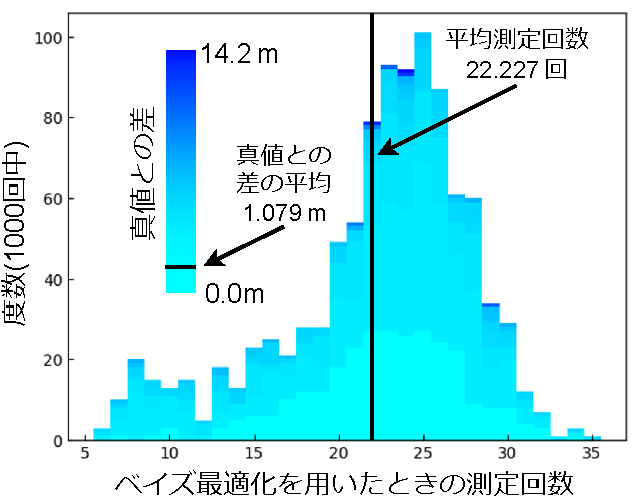
\includegraphics[width=0.71\linewidth]{./figures/material_5_result.pdf}
	\vspace*{-0.3cm}
	\caption{ベイズ最適化を適用したときの結果} \label{fig:result}
\end{figure}
\section{おわりに}

ベイズ最適化を用いて送信機の最適な位置を求める手法を提案し,シミュレーションでその有用性を確認した.
その結果,提案手法は全探索と比較して測定回数を大幅に削減することができた.
しかし,真値とベイズ最適化による最適値の差が出てしまった.
原因として,電波は距離の累乗に比例して減衰するため,ガウス関数のような滑らかな関数が適していなかったためであると考えられる.
そのため,今後は\weq{exp_kernel}の指数カーネルや\weq{sin_kernel}の周期カーネルなどの別のカーネル関数を用いてベイズ最適化を行い,測定回数の削減や真値との差を小さくする.

\printbibliography[title=参考文献]

\end{document}
